\chapter{Potensial Listrik; Penghantar dan Kapasitor}\label{ch:b1:potential-capacitors}

Sebuah medan adalah tiga bilangan di setiap titik; sebuah potensial hanya
satu. Karena gaya elektrostatiknya \omterm{def:b1:work-and-energy:conservative}{konservatif}, seluruh medan sebuah
distribusi muatan dapat dilipat menjadi satu fungsi skalar, yaitu
potensialnya, yang darinya medan itu diperoleh kembali dengan penurunan ---
penghematan yang sama yang mengubah gaya menjadi \omterm{def:b1:work-and-energy:conservative}{energi potensial} dalam
mekanika. Potensial adalah apa yang dibaca voltmeter, apa yang dijaga
sebuah baterai, apa yang mempercepat elektron di dalam sebuah tabung;
permukaan-permukaan tingkatnya memetakan sebuah medan dalam sekali pandang.
Bab ini membangunnya, memakainya pada dipol (model listrik pertama sebuah
molekul), lalu beralih ke dua benda yang menyusun setiap rangkaian:
penghantar, tempat muatan menata dirinya sendiri sehingga medan di dalamnya
lenyap, dan \omterm{def:b1:potential-capacitors:capacitance}{kapasitor}, yang menyimpan muatan dan \omterm{def:b1:kinetic-theory:U}{energi dalam} sebuah medan.

\begin{omfigure}
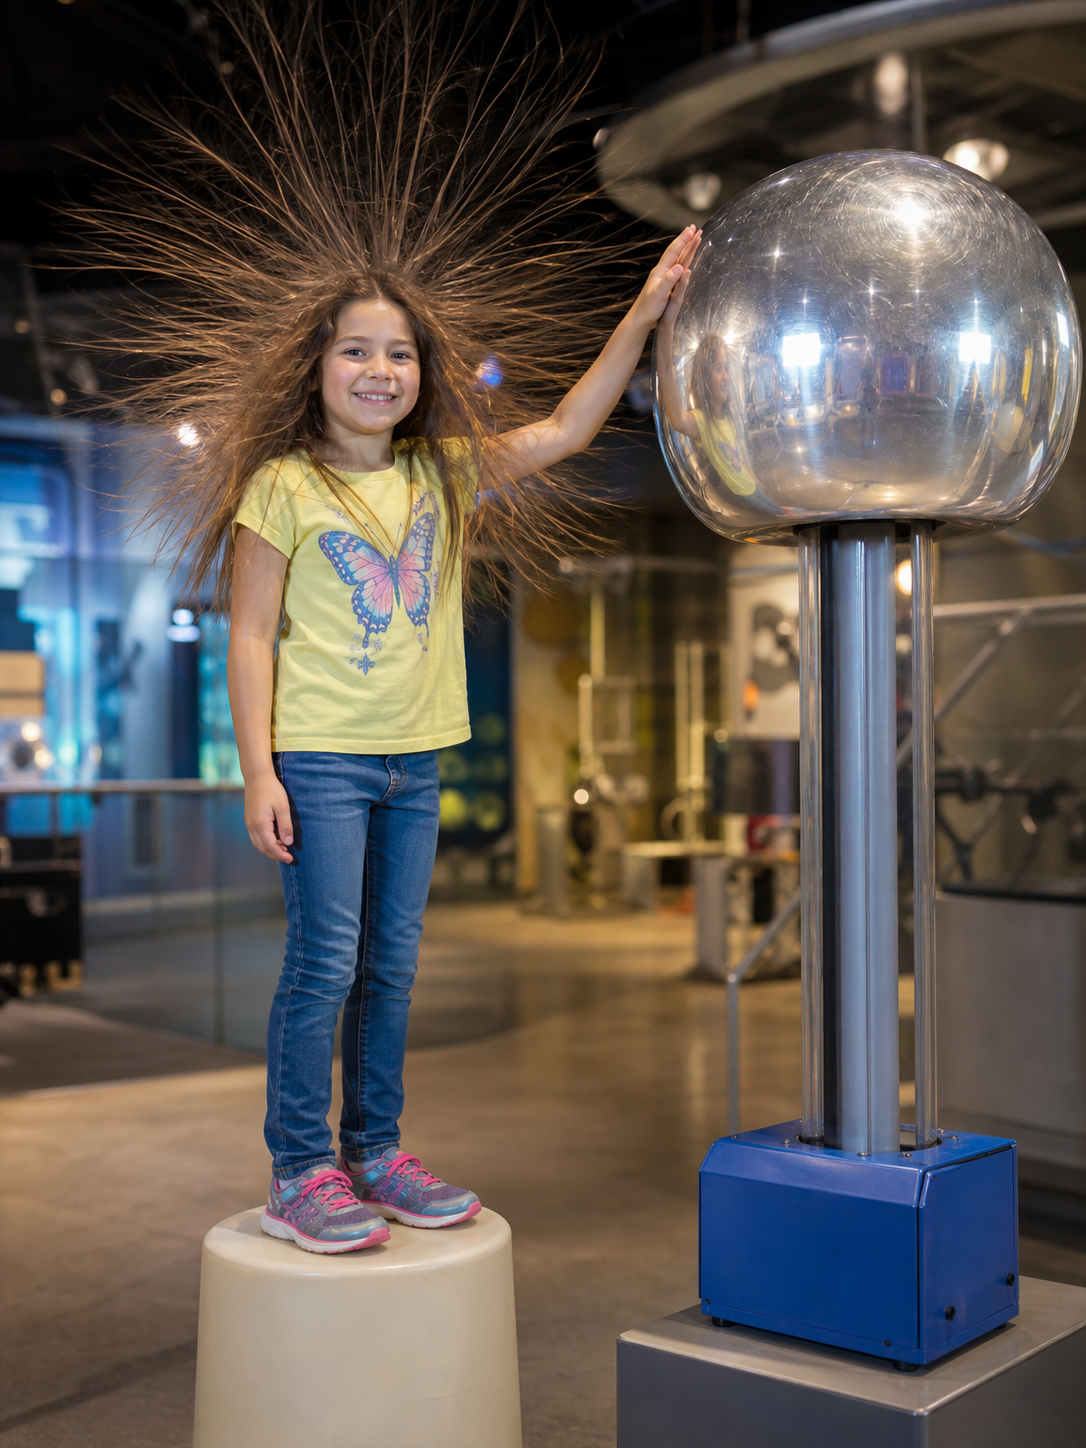
\includegraphics[width=0.34\linewidth]{images/book3/ai/b3-27-van-de-graaff-hair.png}

{\small Dimuati sampai beberapa ratus kilovolt oleh sebuah generator Van de Graaff, seseorang menjadi penghantar ekuipotensial yang rambutnya, semuanya berpotensial sama dan bermuatan sejenis, saling tolak-menolak.}
\end{omfigure}

\section{Potensial elektrostatik}

\begin{theorem}[Medan elektrostatik bersifat konservatif]\label{thm:b1:potential-capacitors:potential}
\index{potensial elektrostatik}\index{volt}\index{sirkulasi}
Terdapat sebuah fungsi skalar $V(M)$, yang disebut \emph{\omterm{thm:b1:potential-capacitors:potential}{potensial
elektrostatik}} (volt, \unit{V}), sedemikian sehingga
\[
\vect E = -\overrightarrow{\operatorname{grad}}\,V , \qquad
V_A - V_B = \int_A^B \vect E\cdot\dd\vect l
\]
menyusuri \omterm{def:b1:point-kinematics:frame}{lintasan} apa pun dari $A$ ke $B$ (\emph{sirkulasi} $\vect E$
dari $A$ ke $B$ tak bergantung pada \omterm{def:b1:point-kinematics:frame}{lintasannya}, dan nol mengelilingi sebuah
gelung tertutup). Bagi sebuah muatan titik $q$ di $O$, $V(M) = \dfrac{q}{4\pi\varepsilon_0\,OM}$
dengan kesepakatan $V(\infty) = 0$; bagi beberapa muatan potensialnya
berjumlah. \omterm{def:b1:work-and-energy:conservative}{Energi potensial} sebuah muatan $q'$ di $M$ adalah $E_p = q'V(M)$, dan
usaha gaya listriknya dari $A$ ke $B$ adalah $q'(V_A - V_B)$.
\end{theorem}

\begin{proof}
Gaya Coulomb sebuah muatan tetap $q$ pada $q'$ berbentuk gravitasi Newton
dengan $-Gm_1m_2$ diganti oleh $qq'/4\pi\varepsilon_0$; perhitungan yang sama
yang memberi $E_p = -Gm_1m_2/r$
(\cref{prop:b1:work-and-energy:eps}) memberi $E_p = qq'/4\pi\varepsilon_0r$:
dibagi $q'$ hasilnya $V$, dan $\vect E = \vect F/q' =
-\overrightarrow{\operatorname{grad}}(E_p)/q'$. Superposisi membawa hasil itu
ke sembarang distribusi; rumus sirkulasinya adalah definisi gradien yang
diintegralkan menyusuri \omterm{def:b1:point-kinematics:frame}{lintasannya}.
\end{proof}

\begin{proposition}[Membaca sebuah potensial]\label{prop:b1:potential-capacitors:reading}
\index{permukaan ekuipotensial}
\begin{enumerate}
  \item \emph{\omterm{prop:b1:potential-capacitors:reading}{Permukaan ekuipotensial}} $V = \text{const}$ di mana-mana
        tegak lurus pada \omterm{def:b1:electrostatics-gauss:field}{garis medannya}, dan medannya menunjuk ke arah
        potensial yang \emph{menurun}.
  \item $|\vect E|$ adalah laju perubahan $V$ menyusuri arah yang paling
        curam: di tempat ekuipotensialnya merapat, medannya kuat.
  \item $V$ terdefinisi sampai sebuah tetapan penjumlah; hanya selisihnya
        (\omterm{def:b1:dc-circuits:voltage}{tegangan}) yang terukur. Tanah atau tak hingga ditetapkan nol
        sebagai kesepakatan.
  \item Dalam \omterm{def:b1:point-kinematics:spherical}{koordinat bola} yang simetrik terhadap $O$, $E_r = -\dd V/
        \dd r$; dalam koordinat kutub $(r, \theta)$ pada sebuah bidang,
        $E_r = -\partial V/\partial r$ dan $E_\theta = -\dfrac1r\,\partial V/\partial\theta$.
\end{enumerate}
\end{proposition}

\begin{proof}
Pada sebuah ekuipotensial $\dd V = -\vect E\cdot\dd\vect l = 0$ bagi setiap
perpindahan di dalam permukaannya, sehingga $\vect E$ normal terhadapnya;
bergerak menyusuri $\vect E$, $\dd V = -E\,\dd l < 0$. Komponen kutubnya menyusul dari
$\dd V = (\partial V/\partial r)\dd r + (\partial V/\partial\theta)\dd\theta$ dan
$\dd\vect l = \dd r\,\vect e_r + r\,\dd\theta\,\vect e_\theta$.
\end{proof}

\begin{omfigure}
\begin{tikzpicture}[font=\small, x=1cm, y=1cm, >=Stealth]
  \begin{scope}
    \foreach \r in {0.6,0.85,1.2,1.7,2.4} \draw[omProp, thick] (0,0) circle (\r);
    \foreach \a in {0,30,...,330} \draw[omDef, ->] (0.25,0) ++({\a}:0) -- ++({\a}:2.7) ;
    \fill[omThm] (0,0) circle (2.5pt) node[below left, font=\footnotesize] {$q > 0$};
    \node[omProp, font=\footnotesize] at (2.05,2.05) {$V = \text{const}$};
    \node[font=\footnotesize] at (0,-3.1) {muatan titik: bola $V \propto 1/r$};
  \end{scope}
  \begin{scope}[xshift=8.4cm]
    \draw[omThm, very thick] (-2.2,-2.2) -- (-2.2,2.2) node[above] {$V_1$};
    \draw[omDef, very thick] (2.2,-2.2) -- (2.2,2.2) node[above] {$V_2 < V_1$};
    \foreach \x in {-1.32,-0.44,0.44,1.32} \draw[omProp, thick] (\x,-2.0) -- (\x,2.0);
    \foreach \y in {-1.5,-0.5,0.5,1.5} \draw[omDef, ->] (-2.1,\y) -- (2.0,\y);
    \node[omProp, font=\footnotesize, anchor=west] at (-1.3,2.25) {ekuipotensial};
    \node[font=\footnotesize] at (0,-3.1) {kapasitor bidang: bidang, $V$ linear dalam $x$};
  \end{scope}
\end{tikzpicture}

{\small Ekuipotensial (jingga) dan \omterm{def:b1:electrostatics-gauss:field}{garis medan} (biru) sebuah muatan
titik dan sebuah \omterm{prop:b1:potential-capacitors:three}{kapasitor bidang}. Garisnya memotong ekuipotensialnya
tegak lurus dan berjalan dari potensial tinggi ke rendah; di tempat
ekuipotensialnya berjejal, medannya kuat.}
\end{omfigure}

\begin{method}[Menghitung sebuah potensial]\label{meth:b1:potential-capacitors:compute}
Jumlahkanlah $\dd q/4\pi\varepsilon_0r$ atas distribusinya (bila jumlahnya
terkelola dan distribusinya berhingga, sehingga $V(\infty) = 0$ masuk
akal), atau integralkanlah $\dd V = -\vect E\cdot\dd\vect l$ menyusuri sebuah
\omterm{def:b1:point-kinematics:frame}{lintasan} yang menyenangkan dari titik yang $V$-nya diketahui, dengan medan
yang diperoleh dari \omterm{thm:b1:electrostatics-gauss:gauss}{hukum Gauss}. Bagi distribusi tak hingga (kawat, bidang)
hanya cara kedua yang berhasil, dan nol $V$-nya harus dipilih di titik berhingga.
\end{method}

\begin{proposition}[Potensial distribusi klasiknya]\label{prop:b1:potential-capacitors:classic}
\begin{enumerate}
  \item Bola berjari-jari $R$ dengan $Q$ dalam volumenya: $V(r) = \dfrac{Q}{4\pi\varepsilon_0r}$
        di luar; $V(r) = \dfrac{Q}{4\pi\varepsilon_0}\,\dfrac{3R^2 - r^2}{2R^3}$
        di dalam, sehingga $V(0) = \tfrac32\,Q/4\pi\varepsilon_0R$. Dengan $Q$ pada permukaannya,
        $V$ seragam di dalam, sama dengan $Q/4\pi\varepsilon_0R$.
  \item Kawat tak hingga $\lambda$: $V(r) = -\dfrac{\lambda}{2\pi\varepsilon_0}\ln\dfrac{r}{r_0}$.
  \item \omterm{prop:b1:potential-capacitors:three}{Kapasitor bidang}, medan $E$ dari keping~1 ke keping~2 yang terpisah
        sejauh $d$: $V$ menurun linear melintasi celahnya dan $V_1 - V_2 = Ed$.
\end{enumerate}
\end{proposition}

\begin{proof}
Integralkanlah $E_r = -\dd V/\dd r$ dengan medan
\cref{prop:b1:electrostatics-gauss:three}, dari tak hingga ke dalam bagi
bolanya (kekontinuan di $R$ menetapkan tetapan dalamnya), dari $r_0$ bagi
kawatnya, melintasi celahnya bagi \omterm{def:b1:potential-capacitors:capacitance}{kapasitornya}.
\end{proof}

\begin{omfigure}
\begin{tikzpicture}
\begin{axis}[omaxis, axis x line=bottom, axis y line=left, width=10cm, height=5.8cm,
    xlabel={$r/R$}, ylabel={},
    xlabel style={at={(axis description cs:0.5,-0.1)}, anchor=north},
    xmin=0, xmax=4, ymin=0, ymax=1.7, xtick={1,2,3}, ytick={0.5,1,1.5}, samples=80, clip=false]
  \addplot[omProp, very thick, domain=0:1] {1.5-0.5*x^2};
  \addplot[omProp, very thick, domain=1:4] {1/x};
  \node[omProp, font=\footnotesize, anchor=east] at (axis cs:3.95,1.5) {$V$ (satuan $Q/4\pi\varepsilon_0R$)};
  \addplot[omDef, thick, dashed, domain=0:1] {x};
  \addplot[omDef, thick, dashed, domain=1:4] {1/x^2};
  \node[omDef, font=\footnotesize, anchor=east] at (axis cs:3.95,1.27) {$E$ (satuan $Q/4\pi\varepsilon_0R^2$)};
  \node[omProp, font=\footnotesize, anchor=west] at (axis cs:0.05,1.58) {$V(0) = \tfrac32\,V(R)$};
\end{axis}
\end{tikzpicture}

{\small Potensial (utuh) dan medan (putus-putus) sebuah bola bermuatan
seragam. Potensialnya kontinu dengan kemiringan yang kontinu; ia
parabolik di dalam, tempat medannya linear, dan sebanding $1/r$ di luar.
Maksimumnya duduk di pusatnya, tempat medannya lenyap --- sebuah maksimum
$V$ adalah titik bermedan nol, bukan sebaliknya.}
\end{omfigure}

\begin{example}[Elektronvolt, sekali lagi]\label{ex:b1:potential-capacitors:eV}
Sebuah elektron yang menyeberangi celah \qty{100}{V} memperoleh $eU = \qty{100}{eV} =
\qty{1.6e-17}{J}$, apa pun bentuk medan di antara kedua
elektrodanya: potensialnya membuat \omterm{def:b1:point-kinematics:frame}{lintasannya} tak relevan
(\cref{def:b1:charged-particles:eV}). Muatan \qty{1}{\micro C} pada jarak
\qty{1}{m} dari muatan lain berpotensial $V = \qty{9}{kV}$ dan pasangannya menyimpan
\qty{9}{mJ}; potensial di pusat sebuah inti emas adalah
\qty{24}{MV} (\cref{exo:b1:potential-capacitors:6}).
\end{example}

\section{Dipol listrik}

\begin{definition}[Dipol listrik]\label{def:b1:potential-capacitors:dipole}
\index{dipol listrik}\index{momen dipol}
Dua muatan berlawanan $-q$ di $N$ dan $+q$ di $P$, yang terpisah sejauh $a = NP$,
membentuk sebuah \emph{dipol listrik} bermomen dipol
$\vect p = q\,\vect{NP}$ (\unit{C.m}), yang menunjuk dari $-$ ke $+$; besaran itu
disebut \emph{momen dipol}. Hampiran dipolnya adalah kajian medannya pada jarak
$r \gg a$. Sebuah molekul yang pusat muatan positif dan negatifnya tak berimpit
(air, $p = \qty{6.2e-30}{C.m}$) merupakan sebuah dipol; sebuah atom netral di
dalam medan menjadi dipol pula (dipol imbasan).
\end{definition}

\begin{proposition}[Medan sebuah dipol]\label{prop:b1:potential-capacitors:dipolefield}
Di $M$ dengan $OM = r \gg a$ ($O$ titik tengah $NP$) dan $\theta$ sudut
antara $\vect p$ dan $\vect{OM}$,
\[
V(M) = \frac{p\cos\theta}{4\pi\varepsilon_0 r^2}, \qquad
E_r = \frac{2p\cos\theta}{4\pi\varepsilon_0r^3}, \qquad
E_\theta = \frac{p\sin\theta}{4\pi\varepsilon_0r^3} .
\]
Medan sebuah dipol meluruh sebanding $1/r^3$, lebih cepat daripada $1/r^2$
sebuah muatan: dari jauh kedua muatannya hampir saling meniadakan, dan yang
tersisa adalah pemisahannya.
\end{proposition}

\begin{proof}
$V = \dfrac{q}{4\pi\varepsilon_0}\Bigl(\dfrac1{PM} - \dfrac1{NM}\Bigr)$ dengan
$PM \approx r - \tfrac a2\cos\theta$ dan $NM \approx r + \tfrac a2\cos\theta$
(proyeksi $\pm\tfrac a2$ pada $\vect{OM}$); sampai orde pertama dalam $a/r$,
$1/PM - 1/NM \approx a\cos\theta/r^2$. Lalu $E_r = -\partial V/\partial r$ dan
$E_\theta = -(1/r)\,\partial V/\partial\theta$.
\end{proof}

\begin{omfigure}
\begin{tikzpicture}[font=\small, x=1cm, y=1cm, >=Stealth]
  \begin{scope}[scale=1.3]
    \fill[omDef] (-0.5,0) circle (2.5pt) node[below left, font=\footnotesize] {$-q$};
    \fill[omThm] (0.5,0) circle (2.5pt) node[below right, font=\footnotesize] {$+q$};
    \draw[->, very thick] (-0.5,0) -- (0.5,0); \node[above, font=\footnotesize] at (0,0.05) {$\vect p$};
    \fill (0,0) circle (1pt); \node[below, font=\footnotesize] at (0,-0.05) {$O$};
    \coordinate (M) at (2.6,1.9);
    \fill (M) circle (1.6pt) node[above right, font=\footnotesize] {$M$};
    \draw[dashed] (0,0) -- (M) node[midway, above left, font=\footnotesize] {$r$};
    \draw[dashed] (-0.5,0) -- (M); \draw[dashed] (0.5,0) -- (M);
    \draw (0.9,0) arc[start angle=0, end angle=36, radius=0.9] node[midway, right, font=\footnotesize] {$\theta$};
    \draw[->, omThm, thick] (M) -- ++(36:0.9) node[right, font=\footnotesize] {$E_r$};
    \draw[->, omThm, thick] (M) -- ++(126:0.6) node[above left, font=\footnotesize] {$E_\theta$};
  \end{scope}
  \begin{scope}[xshift=8.6cm, scale=1.0]
    % field lines: circles through the charges (dipole limit: r = K sin^2 theta)
    \foreach \K in {0.8,1.6,2.6} {
      \draw[omDef, thick, domain=3:177, samples=60, smooth] plot ({\K*sin(\x)*sin(\x)*cos(\x)}, {\K*sin(\x)*sin(\x)*sin(\x)});
      \draw[omDef, thick, domain=183:357, samples=60, smooth] plot ({\K*sin(\x)*sin(\x)*cos(\x)}, {\K*sin(\x)*sin(\x)*sin(\x)});
    }
    % equipotentials r = A sqrt(|cos theta|)
    \foreach \A in {0.9,1.5,2.2} {
      \draw[omProp, thick, domain=-88:88, samples=50, smooth] plot ({\A*sqrt(cos(\x))*cos(\x)}, {\A*sqrt(cos(\x))*sin(\x)});
      \draw[omProp, thick, domain=92:268, samples=50, smooth] plot ({\A*sqrt(-cos(\x))*cos(\x)}, {\A*sqrt(-cos(\x))*sin(\x)});
    }
    \draw[->, very thick] (-0.25,0) -- (0.25,0);
    \node[font=\footnotesize, omProp] at (2.95,0.45) {$V > 0$};
    \node[font=\footnotesize, omProp] at (-2.95,0.45) {$V < 0$};
  \end{scope}
\end{tikzpicture}

{\small Kiri: geometri hampiran dipolnya --- $M$ dilihat dari
pusat $O$ pada jarak $r$ dan sudut $\theta$ dari $\vect p$, dengan komponen
medan radial dan ortoradialnya. Kanan: \omterm{def:b1:electrostatics-gauss:field}{garis medan} (biru,
$r \propto \sin^2\theta$) dan ekuipotensial (jingga, $r \propto
\sqrt{|\cos\theta|}$) sebuah dipol yang menunjuk ke kanan; bidang melalui $O$
yang tegak lurus pada $\vect p$ adalah ekuipotensial $V = 0$.}
\end{omfigure}

\begin{proposition}[Dipol dalam medan luar]\label{prop:b1:potential-capacitors:dipoleinfield}
\index{dipol!momen gaya}\index{dipol!energi}
Sebuah dipol $\vect p$ dalam medan seragam $\vect E$ tak merasakan gaya total,
merasakan \omterm{def:b1:angular-momentum:moment}{momen gaya} $\vect\Gamma = \vect p\wedge\vect E$ yang cenderung
menyearahkannya dengan medannya, dan memiliki \omterm{def:b1:work-and-energy:conservative}{energi potensial} $E_p = -\vect p\cdot\vect E$,
yang minimum ketika searah. Dalam medan tak seragam ia lebih jauh lagi ditarik
ke daerah bermedan kuat (dalam satu dimensi, $F_x = p\,\dd E/\dd x$
bagi dipol yang searah).
\end{proposition}

\begin{proof}
Gaya $\pm q\vect E$ saling meniadakan; momennya terhadap $O$ adalah $\vect{OP}\wedge
q\vect E + \vect{ON}\wedge(-q\vect E) = q\vect{NP}\wedge\vect E$. Energinya:
$qV(P) - qV(N) = -q\,\vect{NP}\cdot\vect E$ bagi medan seragam (karena $V(P)
- V(N) = -\vect E\cdot\vect{NP}$). Tak seragam, searah menyusuri $x$: $F_x =
qE(x + a) - qE(x) \approx qa\,\dd E/\dd x$.
\end{proof}

\begin{example}[Mengapa sisirnya menarik kertasnya]\label{ex:b1:potential-capacitors:comb}
Sebuah sisir bermuatan menciptakan medan yang meluruh dengan jarak; sepotong
kertas yang netral terpolarisasi olehnya (dipol imbasan menyusuri $\vect E$), dan
gaya $p\,\dd E/\dd x$ pada dipol yang searah menariknya ke daerah
bermedan kuat, yaitu sisirnya. Tanda muatan sisirnya tak berperan;
mekanisme yang sama menahan balonnya di dinding dan membuat
seurai air membelok. Bagi molekul air, $pE$ dalam medan \qty{1}{MV/m}
bernilai \qty{6e-24}{J}, $600$ kali lebih kecil daripada $k_BT$ pada suhu ruang:
hanya sedikit penyearahan total yang bertahan terhadap jungkir-balik termalnya
(\cref{exo:b1:potential-capacitors:7}).
\end{example}

\section{Penghantar dalam kesetimbangan elektrostatik}

\begin{theorem}[Sifat sebuah penghantar dalam kesetimbangan]\label{thm:b1:potential-capacitors:conductor}
\index{penghantar dalam kesetimbangan}\index{teorema Coulomb}\index{sangkar Faraday}
Dalam sebuah penghantar yang muatan bebasnya diam:
\begin{enumerate}
  \item $\vect E = \vect 0$ di dalamnya, dan penghantarnya merupakan volume
        ekuipotensial: $V$ seragam di dalamnya dan pada permukaannya.
  \item Setiap muatan total duduk pada permukaannya, dengan rapat permukaan
        $\sigma$; bagian dalamnya netral.
  \item Tepat di luarnya, medannya normal terhadap permukaannya dan bernilai
        $\vect E = \dfrac{\sigma}{\varepsilon_0}\,\vect n$ (\emph{teorema Coulomb}).
  \item Sebuah rongga di dalam penghantar, yang kosong dari muatan, memiliki $\vect E =
        \vect 0$ dan $V$ seragam apa pun yang terjadi di luarnya (\emph{\omterm{thm:b1:potential-capacitors:conductor}{sangkar
        Faraday}}).
\end{enumerate}
\end{theorem}

\begin{proof}
(1) Sebuah medan akan menggerakkan muatan bebasnya: kesetimbangan menuntut $\vect E =
\vect 0$, sehingga $\dd V = 0$ di antara dua titik dalam mana pun; permukaannya
adalah limitnya. (2) \omterm{thm:b1:electrostatics-gauss:gauss}{Hukum Gauss} pada sembarang permukaan tertutup yang
digambar di dalam penghantarnya: fluksnya nol, muatan terlingkupinya nol.
(3) Permukaannya sebuah ekuipotensial, sehingga $\vect E$ tepat di luarnya
normal terhadapnya; sebuah kotak pil yang mengangkangi permukaannya berfluks
$E\,\dd S$ hanya lewat muka luarnya (di dalam $\vect E = \vect 0$) dan bermuatan
$\sigma\,\dd S$. (4) Dinding rongganya sebuah ekuipotensial; sebuah \omterm{def:b1:electrostatics-gauss:field}{garis medan}
di dalam rongganya harus pergi dari dinding ke dinding melintasi sebuah jatuh
potensial --- mustahil pada sebuah ekuipotensial; jadi tak ada garis, tak ada
medan (diterima tanpa bukti dalam bentuk ini).
\end{proof}

\begin{example}[Efek ujung runcing dan penangkal petir]\label{ex:b1:potential-capacitors:point}
\index{efek ujung runcing}
Dua bola berjari-jari $R_1 > R_2$, yang berjauhan dan dihubungkan oleh sebuah
kawat, berbagi $V = Q_i/4\pi\varepsilon_0R_i$ yang sama, sehingga $\sigma_i = Q_i/4\pi R_i^2 = \varepsilon_0V/R_i$:
makin \emph{kecil} \omterm{def:b1:point-kinematics:frenet}{jari-jari kelengkungannya}, makin \emph{besar} muatan
permukaan dan medannya $\sigma/\varepsilon_0 = V/R$. Pada sebuah ujung yang tajam
medannya melampaui nilai dadal udara (\qty{3}{MV/m}) jauh sebelum hal itu
terjadi di tempat lain: udaranya terionisasi dan muatannya merembes pergi
diam-diam. Sebuah penangkal petir bekerja dengan \emph{\omterm{ex:b1:potential-capacitors:point}{efek ujung runcing}}
ini --- ia tak begitu menarik sambarannya melainkan menawarinya sebuah
\omterm{def:b1:point-kinematics:frame}{lintasan}, dan mengalirkan muatan di bawah sebuah awan sebelum ia menumpuk.
\end{example}

\begin{omfigure}
\begin{tikzpicture}[font=\small, x=1cm, y=1cm, >=Stealth]
  % Faraday cage
  \begin{scope}
    \draw[fill=omExo!20, draw=omExo, thick] (-1.6,-1.3) rectangle (1.6,1.3);
    \draw[fill=white, draw=omExo, thick] (-1.0,-0.75) rectangle (1.0,0.75);
    \foreach \y in {-1.0,-0.5,0,0.5,1.0} \draw[omDef, ->] (-3.0,\y) -- (-1.65,\y);
    \foreach \y in {-1.0,-0.5,0,0.5,1.0} \draw[omDef, ->] (1.65,\y) -- (3.0,\y);
    \foreach \y in {-1.0,-0.5,0,0.5,1.0} {\node[omDef, font=\scriptsize] at (-1.75,\y+0.18) {$-$}; \node[omThm, font=\scriptsize] at (1.75,\y+0.18) {$+$};}
    \node[font=\footnotesize] at (0,0) {$\vect E = \vect 0$};
    \node[font=\footnotesize] at (0,-1.85) {penghantar dalam medan luar};
  \end{scope}
  % point effect
  \begin{scope}[xshift=8.4cm]
    \draw[fill=omExo!20, draw=omExo, thick] (-1.2,0) circle (1.2);
    \draw[fill=omExo!20, draw=omExo, thick] (0,0.12) -- (2.4,0.0) -- (0,-0.12) -- cycle;
    \draw[omExo, thick] (2.4,0) circle (0.06);
    \foreach \a in {100,135,170,205,240,275} \draw[omDef, ->] (-1.2,0) ++({\a}:1.25) -- ++({\a}:0.5);
    \foreach \a in {-40,-20,0,20,40} \draw[omDef, ->] (2.4,0) ++({\a}:0.1) -- ++({\a}:1.2);
    \node[font=\footnotesize, omDef] at (-1.2,2.0) {$\sigma$ kecil, $E$ lemah};
    \node[font=\footnotesize, omDef] at (2.6,1.0) {$\sigma$ besar, $E$ kuat};
    \node[font=\footnotesize] at (0.6,-1.85) {$V$ sama di mana-mana: medan $\propto 1/R$};
  \end{scope}
\end{tikzpicture}

{\small Kiri: sebuah penghantar berongga dalam medan luar --- muatan
imbasan pada permukaannya meniadakan medan di dalamnya dan di dalam
rongganya (\omterm{thm:b1:potential-capacitors:conductor}{sangkar Faraday}). Kanan: \omterm{ex:b1:potential-capacitors:point}{efek ujung runcing} --- pada satu
penghantar ekuipotensial muatan permukaan dan medan luarnya terbesar di
tempat kelengkungannya paling tajam.}
\end{omfigure}

\section{Kapasitor}

\begin{definition}[Kapasitansi]\label{def:b1:potential-capacitors:capacitance}
\index{kapasitansi}\index{kapasitor}\index{farad}
Sebuah penghantar terkucil pada potensial $V$ mengemban muatan $Q$
yang sebanding dengan $V$: $Q = CV$, dengan $C$ yang disebut
\emph{kapasitansi}-nya (farad, \unit{F}); bagi sebuah bola $C = 4\pi\varepsilon_0R$.
Yang disebut \emph{kapasitor} adalah sepasang penghantar (\emph{keping}) yang
mengemban muatan berlawanan $\pm Q$ dan saling berhadapan sehingga medannya
terkurung di antara keduanya; kapasitansinya $C = Q/U$ dengan $U = V_1 - V_2$
\omterm{def:b1:dc-circuits:voltage}{tegangan} di antara kedua kepingnya. Lambang dan hukum rangkaian $i = C\,\dd u/\dd t$
telah dipakai dalam \cref{ch:b1:transient-regimes}.
\end{definition}

\begin{proposition}[Tiga kapasitor]\label{prop:b1:potential-capacitors:three}
\index{kapasitor bidang}\index{kapasitor bola}\index{kapasitor silinder}
\begin{enumerate}
  \item Bidang: keping berluas $S$ yang terpisah sejauh $d \ll \sqrt S$:
        $C = \dfrac{\varepsilon_0S}{d}$.
  \item Bola: bola sepusat berjari-jari $R_1 < R_2$:
        $C = \dfrac{4\pi\varepsilon_0R_1R_2}{R_2 - R_1}$.
  \item Silinder (sesumbu), berjari-jari $a < b$, panjang $L \gg b$:
        $C = \dfrac{2\pi\varepsilon_0L}{\ln(b/a)}$.
\end{enumerate}
Mengisi celahnya dengan sebuah isolator berpermitivitas nisbi
$\varepsilon_r$ melipatkan $C$ dengan $\varepsilon_r$ (molekul dielektriknya
terpolarisasi dan melemahkan medannya, $\varepsilon_r = 2$ sampai $10$ bagi
plastik dan kaca biasa, $80$ bagi air).
\end{proposition}

\begin{proof}
Dalam tiap kasusnya medan di antara kedua kepingnya adalah medan
\cref{prop:b1:electrostatics-gauss:three}: $E = \sigma/\varepsilon_0 = Q/\varepsilon_0S$,
$U = Ed$; $E = Q/4\pi\varepsilon_0r^2$, $U = \int_{R_1}^{R_2}E\,\dd r = \dfrac{Q}{4\pi\varepsilon_0}
\Bigl(\dfrac1{R_1} - \dfrac1{R_2}\Bigr)$; $E = Q/2\pi\varepsilon_0Lr$, $U =
\dfrac{Q}{2\pi\varepsilon_0L}\ln\dfrac ba$. Bagilah $Q$ dengan $U$. Faktor
dielektriknya diterima tanpa bukti.
\end{proof}

\begin{theorem}[Energi sebuah kapasitor]\label{thm:b1:potential-capacitors:energy}
\index{energi sebuah kapasitor}\index{rapat energi medan listrik}
Sebuah \omterm{def:b1:potential-capacitors:capacitance}{kapasitor} yang bermuatan $Q$ di bawah $U$ menyimpan
\[
W = \tfrac12 CU^2 = \tfrac12 QU = \frac{Q^2}{2C} ,
\]
yaitu usaha yang diperlukan untuk membawa muatannya dari satu keping ke
keping yang lain melawan \omterm{def:b1:dc-circuits:voltage}{tegangan} yang membesar. Dalam \omterm{prop:b1:potential-capacitors:three}{kapasitor bidang}
$W = \tfrac12\varepsilon_0E^2
\times Sd$: energinya ada di dalam medannya, pada rapat $\tfrac12\varepsilon_0E^2$
tiap satuan volume --- sebuah pernyataan yang berlaku bagi setiap medan
elektrostatik.
\end{theorem}

\begin{proof}
Memindahkan $\dd q$ dari keping negatif ke keping positif ketika muatannya
$q$ menelan $\dd W = (q/C)\,\dd q$; integralkan dari $0$ sampai $Q$. Lalu
substitusikan $C = \varepsilon_0S/d$ dan $U = Ed$; rapat umumnya diterima tanpa bukti.
\end{proof}

\begin{example}[Tiga kapasitor dan energinya]\label{ex:b1:potential-capacitors:energies}
Sepasang kertas timah seluas satu meter persegi yang terpisah \qty{1}{mm}: $C = 8.85 \times 10^{-12}/
10^{-3} = \qty{8.9}{nF}$ --- \omterm{def:b1:potential-capacitors:capacitance}{farad} memang satuan yang raksasa. Sebuah defibrilator
\qty{150}{\micro F} pada \qty{2}{kV}: \qty{300}{J}, disalurkan dalam beberapa milisekon.
Sebuah superkapasitor \qty{3000}{F} pada \qty{2.7}{V}: \qty{11}{kJ} dalam sebuah
kaleng sebesar botol limun --- \omterm{def:b1:potential-capacitors:capacitance}{kapasitansinya} datang dari celah $d$ berukuran
molekul dan $S$ berliang yang luar biasa besar. Rapat energi sebuah medan pada
dadal udara, $\tfrac12\varepsilon_0(3 \times 10^6)^2 = \qty{40}{J/m^3}$, adalah
sebabnya \omterm{def:b1:potential-capacitors:capacitance}{kapasitor} menyimpan begitu sedikit dibandingkan dengan baterai.
\end{example}

\begin{omfigure}
\begin{tikzpicture}[font=\small, x=1cm, y=1cm, >=Stealth]
  \begin{scope}
    \draw[omThm, very thick] (-1.5,1) -- (1.5,1) node[right, font=\footnotesize] {$+Q$, $V_1$};
    \draw[omDef, very thick] (-1.5,-1) -- (1.5,-1) node[right, font=\footnotesize] {$-Q$, $V_2$};
    \foreach \x in {-1.1,-0.55,0,0.55,1.1} \draw[omProp, ->] (\x,0.9) -- (\x,-0.85);
    \draw[omProp, dashed] (-1.55,0.9) .. controls (-2.2,0.5) and (-2.2,-0.5) .. (-1.55,-0.85);
    \draw[omProp, dashed] (1.55,0.9) .. controls (2.2,0.5) and (2.2,-0.5) .. (1.55,-0.85);
    \draw[<->] (-2.6,1) -- (-2.6,-1) node[midway, left, font=\footnotesize] {$d$};
    \node[font=\footnotesize] at (0,-1.7) {bidang: $C = \varepsilon_0S/d$};
    \node[font=\footnotesize, omProp, fill=white, inner sep=1.5pt] at (0.27,0.3) {$E = U/d$};
  \end{scope}
  \begin{scope}[xshift=6.2cm]
    \draw[omDef, very thick] (0,0) circle (1.3);
    \draw[omThm, very thick, fill=omThm!15] (0,0) circle (0.55);
    \foreach \a in {0,60,...,300} \draw[omProp, ->] (0,0) ++({\a}:0.6) -- ++({\a}:0.6);
    \draw[<->] (0,0) -- (225:0.55) node[midway, above left, font=\scriptsize] {$R_1$};
    \draw[<->] (0,0) -- (-20:1.3) node[pos=0.75, below, font=\scriptsize] {$R_2$};
    \node[font=\footnotesize] at (0,-1.7) {bola (atau silinder, dalam penampang)};
  \end{scope}
  \begin{scope}[xshift=11.2cm]
    \fill[omExo!25] (-1.2,-0.95) rectangle (1.2,0.95);
    \draw[omThm, very thick] (-1.2,1) -- (1.2,1);
    \draw[omDef, very thick] (-1.2,-1) -- (1.2,-1);
    \node[font=\footnotesize] at (0,0) {$\varepsilon_r$};
    \node[font=\footnotesize] at (0,-1.7) {dielektrik: $C \to \varepsilon_rC$};
  \end{scope}
\end{tikzpicture}

{\small \omterm{prop:b1:potential-capacitors:three}{Kapasitor bidang}, bola dan berisi dielektrik. Medannya
(jingga) terkurung di antara kedua kepingnya kecuali kebocoran di
tepinya, yang diabaikan bila $d$ kecil; energi $\tfrac12\varepsilon_0E^2$ tiap
satuan volume tinggal di dalam medan itu.}
\end{omfigure}

\begin{remark}[Kapasitor yang dirangkai]\label{rem:b1:potential-capacitors:association}
Dalam rangkaian paralel ($U$ sama) muatannya berjumlah: $C = C_1 + C_2$; dalam
rangkaian seri ($Q$ sama) \omterm{def:b1:dc-circuits:voltage}{tegangannya} berjumlah: $1/C = 1/C_1 + 1/C_2$ ---
kebalikan dari \omterm{def:b1:dc-circuits:resistor}{resistor}, karena $C$ mengukur sebuah kemudahan (muatan tiap
volt) sedangkan $R$ mengukur sebuah kesukaran. Aturan ini menyusul dari
$Q = CU$ dan hukum rangkaian \cref{ch:b1:dc-circuits}.
\end{remark}

\section{Latihan}

\begin{exercise}[$\star$]\label{exo:b1:potential-capacitors:1}
Potensial pada jarak \qty{1.0}{m} dari muatan \qty{1.0}{\micro C}; energi yang
diperlukan untuk membawa muatan \qty{1.0}{\micro C} kedua dari tak hingga ke
titik itu; kelajuan saat ia terlontar bila dilepaskan, jika massanya \qty{1}{g}.
\end{exercise}

\begin{exercise}[$\star$]\label{exo:b1:potential-capacitors:2}
Keping yang terpisah \qty{1.0}{mm} di bawah \qty{100}{V}: medannya; \omterm{thm:b1:work-and-energy:ke}{energi
kinetik} dan kelajuan yang diperoleh sebuah elektron yang menyeberangi celahnya
dari keadaan diam; waktu terbangnya.
\end{exercise}

\begin{exercise}[$\star$]\label{exo:b1:potential-capacitors:3}
Pada sebuah peta ekuipotensial yang digambar tiap \qty{10}{V}, garisnya
terpisah \qty{2}{mm} dekat $A$ dan \qty{8}{mm} dekat $B$. Medan di $A$
dan di $B$; ke mana medannya menunjuk relatif terhadap potensial yang
membesar; ke mana sebuah elektron dipercepat?
\end{exercise}

\begin{exercise}[$\star$]\label{exo:b1:potential-capacitors:4}
Sebuah bola Van de Graaff berjari-jari \qty{15}{cm} dimuati sampai \qty{200}{kV}.
\omterm{def:b1:potential-capacitors:capacitance}{Kapasitansi}, muatan, medan pada permukaannya. Potensial maksimum sebelum
udara di sekitarnya dadal (\qty{3}{MV/m}).
\end{exercise}

\begin{exercise}[$\star\star$]\label{exo:b1:potential-capacitors:5}
Potensial pada sumbu sebuah cincin berjari-jari $R$ dan bermuatan $Q$; peroleh
kembali medan aksialnya dengan penurunan. Serupa bagi cakram bermuatan seragam
(pakailah \cref{exo:b1:electrostatics-gauss:5}): $V(z) = \dfrac{\sigma}{2\varepsilon_0}
\bigl(\sqrt{z^2 + R^2} - z\bigr)$.
\end{exercise}

\begin{exercise}[$\star\star$]\label{exo:b1:potential-capacitors:6}
Turunkanlah potensial di dalam sebuah bola bermuatan seragam dari medannya.
Potensial di pusat sebuah inti emas ($Z = 79$, $R = \qty{7.0}{fm}$);
energi yang diperlukan sebuah proton untuk mencapai pusatnya dari jauh, dalam
\unit{MeV}; ulaslah partikel alfa \qty{5}{MeV} milik Rutherford.
\end{exercise}

\begin{exercise}[$\star\star$]\label{exo:b1:potential-capacitors:7}
Molekul air, $p = \qty{6.2e-30}{C.m}$. Medan yang diciptakannya pada \qty{1.0}{nm}
menyusuri sumbunya dan tegak lurus terhadapnya; \omterm{def:b1:angular-momentum:moment}{momen gaya} dan selisih energi
antara kedudukan searah dan berlawanan arah dalam $E = \qty{1.0}{MV/m}$;
bandingkan dengan $k_BT$ pada \qty{300}{K}. Medan sebuah ion natrium pada
\qty{0.3}{nm} dan energi dipol airnya yang searah di dalamnya (hidrasi).
\end{exercise}

\begin{exercise}[$\star\star$]\label{exo:b1:potential-capacitors:8}
Sebuah bola penghantar berjari-jari \qty{1.0}{cm} di udara: muatan dan potensial
maksimum sebelum dadal. Dua bola penghantar, $R_1 = \qty{10}{cm}$
dan $R_2 = \qty{1.0}{mm}$, dihubungkan oleh kawat tipis dan dinaikkan sampai
\qty{20}{kV}: medan permukaan masing-masing; yang mana melucut ke udara?
\end{exercise}

\begin{exercise}[$\star\star$]\label{exo:b1:potential-capacitors:9}
\omterm{def:b1:potential-capacitors:capacitance}{Kapasitansi}: dua kertas timah \qty{1.0}{m^2} yang terpisah \qty{10}{\micro m}
dengan lapisan polimer $\varepsilon_r = 2.2$ (sebuah \omterm{def:b1:potential-capacitors:capacitance}{kapasitor} lapisan); kertas
timah yang sama digulung --- apakah penggulungan mengubah $C$? Energinya pada
\qty{400}{V}. Sebuah \omterm{def:b1:potential-capacitors:capacitance}{kapasitor} \qty{150}{\micro F} pada \qty{2.0}{kV}
(defibrilator): muatan, energi, \omterm{thm:b1:sinusoidal-impedance:power}{daya rata-rata} bila disalurkan dalam \qty{5}{ms}.
\end{exercise}

\begin{exercise}[$\star\star\star$]\label{exo:b1:potential-capacitors:10}
\emph{\omterm{prop:b1:potential-capacitors:three}{Kapasitor bola} dan silinder.} (a) Turunkanlah $C$ bagi bola sepusat
dan periksalah bahwa untuk $R_2 - R_1 = d \ll R_1$ ia menyusut menjadi
rumus bidangnya, dan untuk $R_2 \to \infty$ menjadi bola terkucilnya.
(b) Kabel sesumbu, $a = \qty{0.5}{mm}$, $b = \qty{2.5}{mm}$, polietilena
$\varepsilon_r = 2.3$: \omterm{def:b1:potential-capacitors:capacitance}{kapasitansi} tiap meter (bandingkan dengan \qty{100}{pF/m}
kabel biasa). (c) Medan pada penghantar dalamnya di bawah
\qty{1}{kV}; amankah?
\end{exercise}

\begin{exercise}[$\star\star\star$]\label{exo:b1:potential-capacitors:11}
\emph{Energi di dalam medannya.} (a) Energi sebuah bola penghantar bermuatan
($Q$, $R$) dari $Q^2/2C$. (b) Samakan dengan energi diam elektron
$m_ec^2 = \qty{0.511}{MeV}$ lalu selesaikan untuk $R$: ``jari-jari elektron
klasik'' (sampai sebuah faktor). (c) Sebuah \omterm{prop:b1:potential-capacitors:three}{kapasitor bidang} terkucil bermuatan
$Q$ kepingnya ditarik dari $d$ menjadi $2d$: perubahan energi tersimpannya, dan
gaya antara kedua kepingnya yang disimpulkan darinya; periksalah terhadap
\cref{exo:b1:electrostatics-gauss:8}. (d) Serupa dengan \omterm{def:b1:potential-capacitors:capacitance}{kapasitornya} dijaga
pada $U$ tetap oleh sebuah baterai: perubahan energinya, dan ke mana selisihnya pergi.
\end{exercise}

\begin{exercise}[$\star\star\star$]\label{exo:b1:potential-capacitors:12}
\emph{Energi Coulomb sebuah inti.} (a) Bangunlah sebuah bola bermuatan
seragam ($Q$, $R$) kulit demi kulit lalu tunjukkan bahwa energi elektrostatiknya
adalah $W = \dfrac{3Q^2}{20\pi\varepsilon_0R}$. (b) Uranium-238: $Z = 92$, $R =
\qty{7.4}{fm}$: $W$ dalam \unit{MeV}. (c) Belahlah menjadi dua serpihan sama besar
($Z/2$, $A/2$, jari-jari $R/2^{1/3}$) yang berjauhan: energi Coulomb yang dilepaskan.
(d) Energi fisi yang terukur kira-kira \qty{200}{MeV}: apa yang melawan
keuntungan Coulombnya?
\end{exercise}

\begin{omfigure}
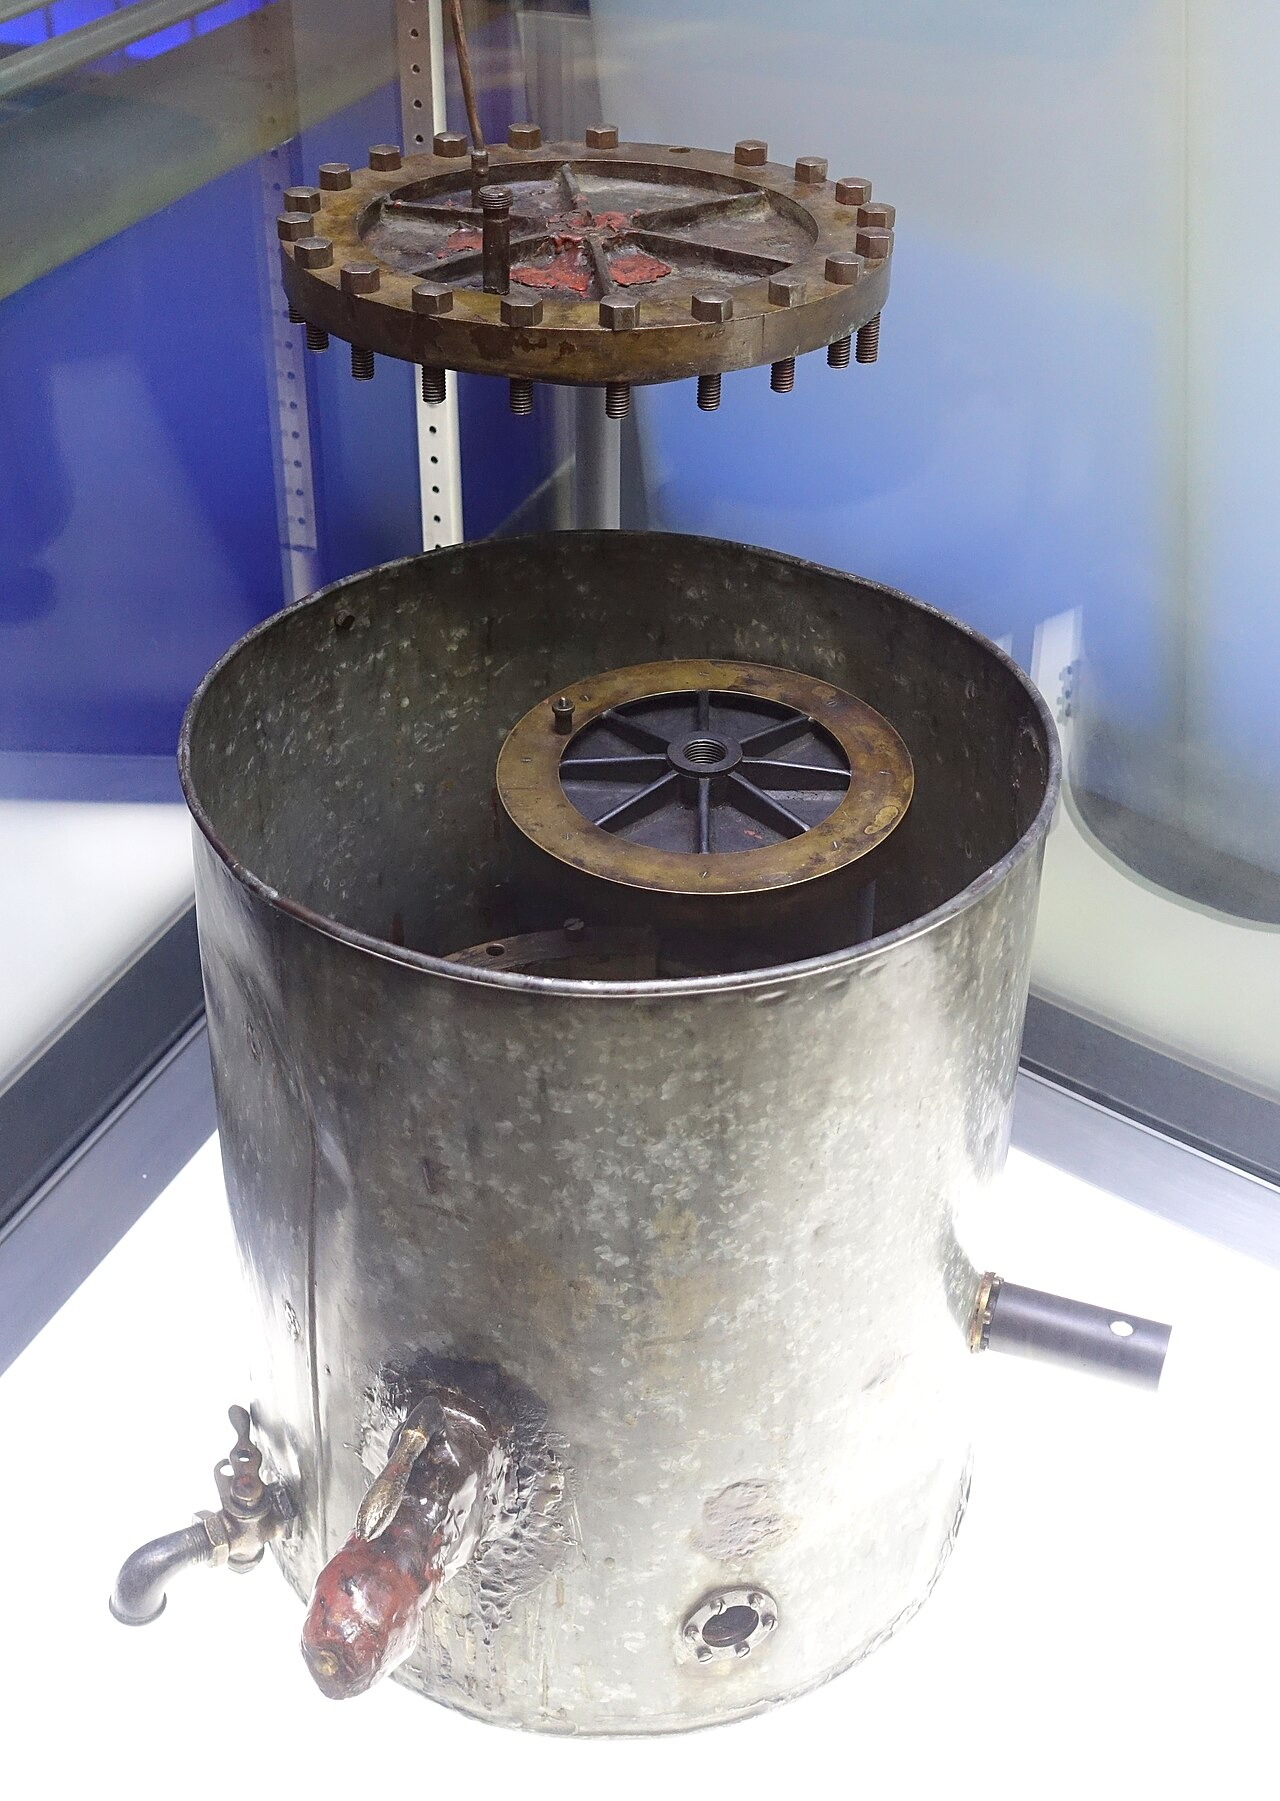
\includegraphics[width=0.36\linewidth]{images/book3/millikan-apparatus.jpg}

{\small Peranti tetes minyak Millikan, kira-kira 1916 (Museum Sains dan Industri, Chicago): bilik kuningannya memuat kedua keping mendatar yang di antaranya tetesnya diamati.}
\end{omfigure}

\section{Soal: Tetes minyak Millikan}

\begin{problem}[{Soal akhir pekan --- menimbang muatan elektron dengan
setetes minyak: Stokes, kapasitor bidang, dan sebuah tabel angka yang
menolak menjadi apa pun kecuali kelipatan satu bilangan}]
\label{pb:b1:potential-capacitors:1}
Tetes minyak disemprotkan di antara dua keping mendatar yang terpisah $d = \qty{16}{mm}$,
berdiameter \qty{20}{cm}, lalu diamati lewat sebuah \omterm{def:b1:optical-instruments:microscope}{mikroskop}.
Data: massa jenis minyak $\rho = \qty{900}{kg/m^3}$, massa jenis udara
\qty{1.2}{kg/m^3}, kekentalan udara $\eta = \qty{1.8e-5}{Pa.s}$, $g =
\qty{9.8}{m/s^2}$, $\varepsilon_0 = \qty{8.85e-12}{F/m}$. Sebuah bola kecil
berjari-jari $r$ yang bergerak dengan $v$ di udara merasakan seretan Stokes $6\pi\eta rv$.

\medskip
\noindent\textbf{Bagian I --- Tetes yang jatuh.}
\begin{enumerate}
  \item Gaya pada sebuah tetes yang jatuh tanpa \omterm{def:b1:dc-circuits:voltage}{tegangan} terpasang; tunjukkan
        bahwa ia mencapai kelajuan terminal $v_1 = 2\rho gr^2/9\eta$ (abaikan
        \omterm{thm:b1:fluid-statics:archimedes}{gaya apung} udaranya --- benarkan).
  \item Sebuah tetes jatuh \qty{1.0}{mm} dalam \qty{10}{s}: jari-jari dan massanya.
  \item \omterm{def:b1:transient-regimes:firstorder}{Tetapan waktu} pendekatan ke $v_1$; jarak yang ditempuh
        sementara itu. Pernahkah tetesnya terlihat dipercepat?
  \item Bilangan Reynolds $\rho_{\text{udara}}v_1r/\eta$ geraknya: sahkah
        \omterm{prop:b1:newton-dynamics:drag}{hukum Stokes}?
  \item Mengapa tetesnya harus sekecil itu? (Bandingkan beratnya dengan
        gaya listrik pada satu \omterm{def:b1:electrostatics-gauss:charge}{muatan elementer} dalam medan
        \qty{3e5}{V/m}.)
  \item Tetesnya terlihat sedikit bergetar di sekitar jatuh rata-ratanya: apa
        ini, dan mengapa ia membatasi ketelitiannya?
\end{enumerate}

\medskip
\noindent\textbf{Bagian II --- Medannya.}
Sebuah \omterm{def:b1:dc-circuits:voltage}{tegangan} $U$ dipasang, keping atasnya positif.
\begin{enumerate}[resume]
  \item Medan di antara kedua kepingnya untuk $U = \qty{5.0}{kV}$; mengapa ia
        seragam, dan apa ekuipotensialnya?
  \item \omterm{def:b1:potential-capacitors:capacitance}{Kapasitansi} kedua kepingnya, muatan padanya pada \qty{5.0}{kV}, dan
        energi tersimpannya.
  \item Tetes pertanyaan~2 tertahan diam untuk $U_0 = \qty{1080}{V}$:
        tanda dan nilai muatannya, dalam coulomb dan dalam satuan $e$.
  \item Dengan $U = \qty{5.0}{kV}$ tetes yang sama naik dengan $v_2$: tunjukkan
        bahwa $q = 6\pi\eta r(v_1 + v_2)d/U$ lalu hitunglah $v_2$.
  \item Mengapa mengukur waktu naik dan turun lebih baik daripada memburu
        \omterm{def:b1:dc-circuits:voltage}{tegangan} penyeimbangnya?
  \item \omterm{def:b1:work-and-energy:conservative}{Energi potensial} muatan tetesnya di antara kedua kepingnya pada
        \qty{5}{kV}, dan energi yang dilesapkan seretan selama sebuah kenaikan
        \qty{1}{cm}.
\end{enumerate}

\medskip
\noindent\textbf{Bagian III --- Tabel muatannya.}
Dipaparkan pada sumber sinar-X yang lemah di antara pengukuran, tetes yang sama
berubah muatannya; pengukuran berturut-turut memberi (dalam $10^{-19}$~C):
$4.80$, $8.01$, $6.42$, $3.19$, $9.63$.
\begin{enumerate}[resume]
  \item Tunjukkan bahwa kelimanya dekat pada kelipatan bulat satu
        besaran, lalu berikan bilangan bulatnya.
  \item Taksiran terbaik \omterm{def:b1:electrostatics-gauss:charge}{muatan elementer} dari kelima nilainya; ketakpastian
        baku reratanya (\cref{ch:b1:units-dimensions}).
  \item Mengapa muatannya berubah sebanyak bilangan bulat $e$ di antara
        pengukuran?
  \item Tunjukkan bahwa, dalam metode ini, $q \propto \eta^{3/2}$: sebesar apa
        galat $1\%$ pada kekentalannya menggeser $e$? (Nilai asli Millikan
        $0.6\%$ terlalu rendah, justru karena sebab ini.)
  \item Kuark mengemban $\pm e/3$ dan $\pm 2e/3$: mengapa tak pernah ada tetes
        minyak yang memperlihatkan sepertiga $e$?
  \item Tetapan Faraday, yaitu muatan satu \omterm{def:b1:kinetic-theory:scales}{mol} elektron, adalah
        $F = \qty{96485}{C/mol}$: simpulkanlah bilangan Avogadro.
  \item Thomson telah mengukur $e/m_e = \qty{1.76e11}{C/kg}$ bagi
        elektron: simpulkanlah massanya, lalu bandingkan dengan sebuah atom
        hidrogen (\qty{1.67e-27}{kg}).
\end{enumerate}

\medskip
\noindent\textbf{Bagian IV --- Perantinya, lewat potensialnya.}
\begin{enumerate}[resume]
  \item Sketsalah ekuipotensial dan \omterm{def:b1:electrostatics-gauss:field}{garis medan} di antara kedua kepingnya,
        termasuk kebocoran dekat tepinya; benarkan pengabaiannya.
  \item Sebuah tetes bermuatan positif pada ketinggian $z$ di atas keping bawah
        (pada \qty{0}{V}): \omterm{def:b1:work-and-energy:conservative}{energi potensialnya} sebagai fungsi $z$; \omterm{def:b1:work-and-energy:conservative}{energi
        potensial} totalnya termasuk gravitasi; syarat pada $U$ bagi titik diamnya.
  \item Bandingkan energi muatan tetesnya (pertanyaan~12) dengan
        energi yang tersimpan dalam \omterm{def:b1:potential-capacitors:capacitance}{kapasitornya}: apakah tetesnya mengganggu medannya?
  \item \omterm{def:b1:dc-circuits:voltage}{Tegangannya} dibalik (keping bawah positif) dengan
        $U = \qty{5.0}{kV}$: apa yang dilakukan tetes pertanyaan~9, dan pada
        kelajuan berapa?
  \item Sebutir debu \qty{1}{\micro g} yang mengemban $10^4e$ dalam medan yang
        sama: nisbah gaya listrik terhadap beratnya; mengapa butiran seperti itu
        tak dapat dilayangkan dan mengapa Millikan memilih kabut minyak.
  \item Ringkaslah: apa yang diukur (tiga kali), apa yang disimpulkan,
        dengan ketakpastian berapa, dan dua tetapan mana yang menyusul darinya.
\end{enumerate}
\end{problem}
